\section{Рекуррентные нейронные сети}

Что же делает рекуррентные сети такими особенными? Вопиющим 
ограничением классических нейронных сетей, рассмотренных ранее 
(а также сверточных нейронных сетей) 
является то, что их API слишком ограничен: 
они принимают на вход вектор фиксированного размера (например, изображение) 
и возвращают вектор фиксированного размера (например, вероятности 
различных классов). Более того, эти модели выполняют заданное отображение за 
фиксированное количество вычислительных шагов (например, количество слоев в модели). 
Основная причина, по которой рекуррентные нейронные сети настолько интересны 
заключается в том, что они позволяют нам работать с \textit{последовательностями} 
векторов: последовательность входных данных, выходных данных, или вообще и того, 
и другого. Рассмотрим несколько примеров:

\begin{figure}[h!]
    \centering
    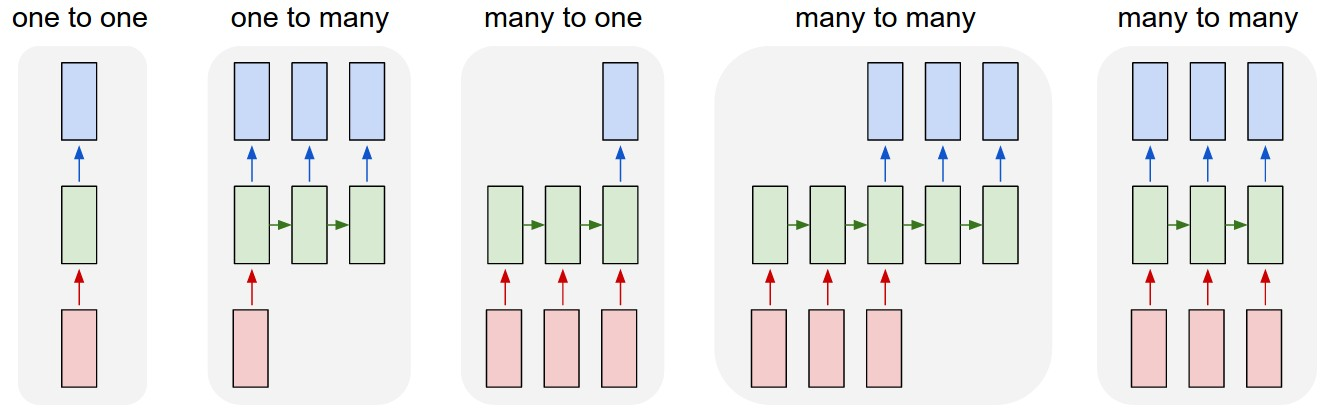
\includegraphics[width=1\textwidth, keepaspectratio]{rnn_sequences}
    \caption{Каждый прямоугольник представляет собой вектор, а стрелки - функции (например, 
    матричное умножение). Векторы входных данных представлены красным цветом, выходных - синим, 
    а зеленые содержат в себе состояние RNN (подробнее об этом далее). Слева направо: 
    (1) Классический метод обработки без RNN, на основании входа конечного размера производит 
    вывод конечного размера (например, классификация изображений). (2) Последовательность 
    в качестве выхода (например, описание изображений). (3) Последовательность в качестве входа 
    (например, анализ эмоциональной окраски, при котором заданное предложение 
    классифицируется как выражающее положительное или негативное настроение). (4) 
    Последовательность в качестве как входа, так и выхода (например, машинный перевод: 
    RNN считывает предложение на английском языке и возвращает его перевод на 
    французском языке). (5) Синхронизированная последовательность в качестве как входа, 
    так и выхода (например, классификация видео, где мы хотим назвать каждый кадр видео). 
    Заметим, что ни в одном из случаев на последовательности длин не наклыдывается 
    никаких предварительных ограничений, т.к. рекуррентное преобразование (зеленое) 
    фиксированно и может применяться сколько угодно раз.}
    \label{fig:rnn_sequences}
\end{figure}

Очевидно, что режим работы с последовательностями гораздо более мощный, по сравнению 
с фиксированными сетями, которые изначально обречены фиксированным количеством 
вычислительных шагов. По своей сути, RNN описывают программы. Вообще говоря, 
если проводить аналогию с универсальными теоремами аппроксимации, то известно, что 
RNN Тьюринг-полны в том смысле, что они могут симулировать поведение произвольных 
программ \cite{karpathy}. Функции, вычислимые машиной Тьюринга, дискретны, и потому 
эти результаты относятся к точной реализации функции, а не к аппроксимациям. 
Когда РНС используется как машина Тьюринга, она принимает на входе двоичную 
последовательность, а ее выходы можно дискретизировать для получения двоичного результата. В таких
предположениях можно вычислить любую функцию с помощью одной конкретной
РНС конечного размера. «Входом» машины Тьюринга является спецификация вычисляемой
функции, поэтому той же сети, которая моделирует машину Тьюринга, достаточно
для решения всех задач \cite{Goodfellow-et-al-2016}.
\begin{center}
    \textit{Если обучение классических нейронных сетей можно назвать оптимизацией над 
    функциями, то обучение рекуррентных сетей можно назвать оптимизацией над программами.}
\end{center}

\noindent\textbf{Примечание} \hspace{10pt} Несмотря на то, что классические RNN сами по себе являются очень интересными, 
они обычно служат, своего рода, переходной ступенью к пониманию более 
продвинутых моделей, таких как LSTM и трансформеры (см. главы 3.2.1 и 4):

\begin{figure}[h!]
    \centering
    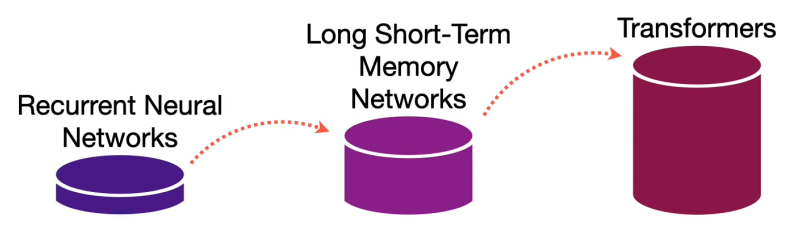
\includegraphics[width=0.8\textwidth, keepaspectratio]{RNN-steps}
    \caption{\cite{statquest_ml_series}}
    \label{fig:RNN-steps}
\end{figure}

\newpage

\subsection{Истоки RNN}

\subsubsection{Архитектура рекуррентной нейронной сети}

Как же рекуррентным нейронным сетям удается работать с последовательностями 
произвольных размеров? У них это получается благодаря циклам, встроенным 
в них, позволяющим сохранять информацию.

\begin{figure}[h!]
    \centering
    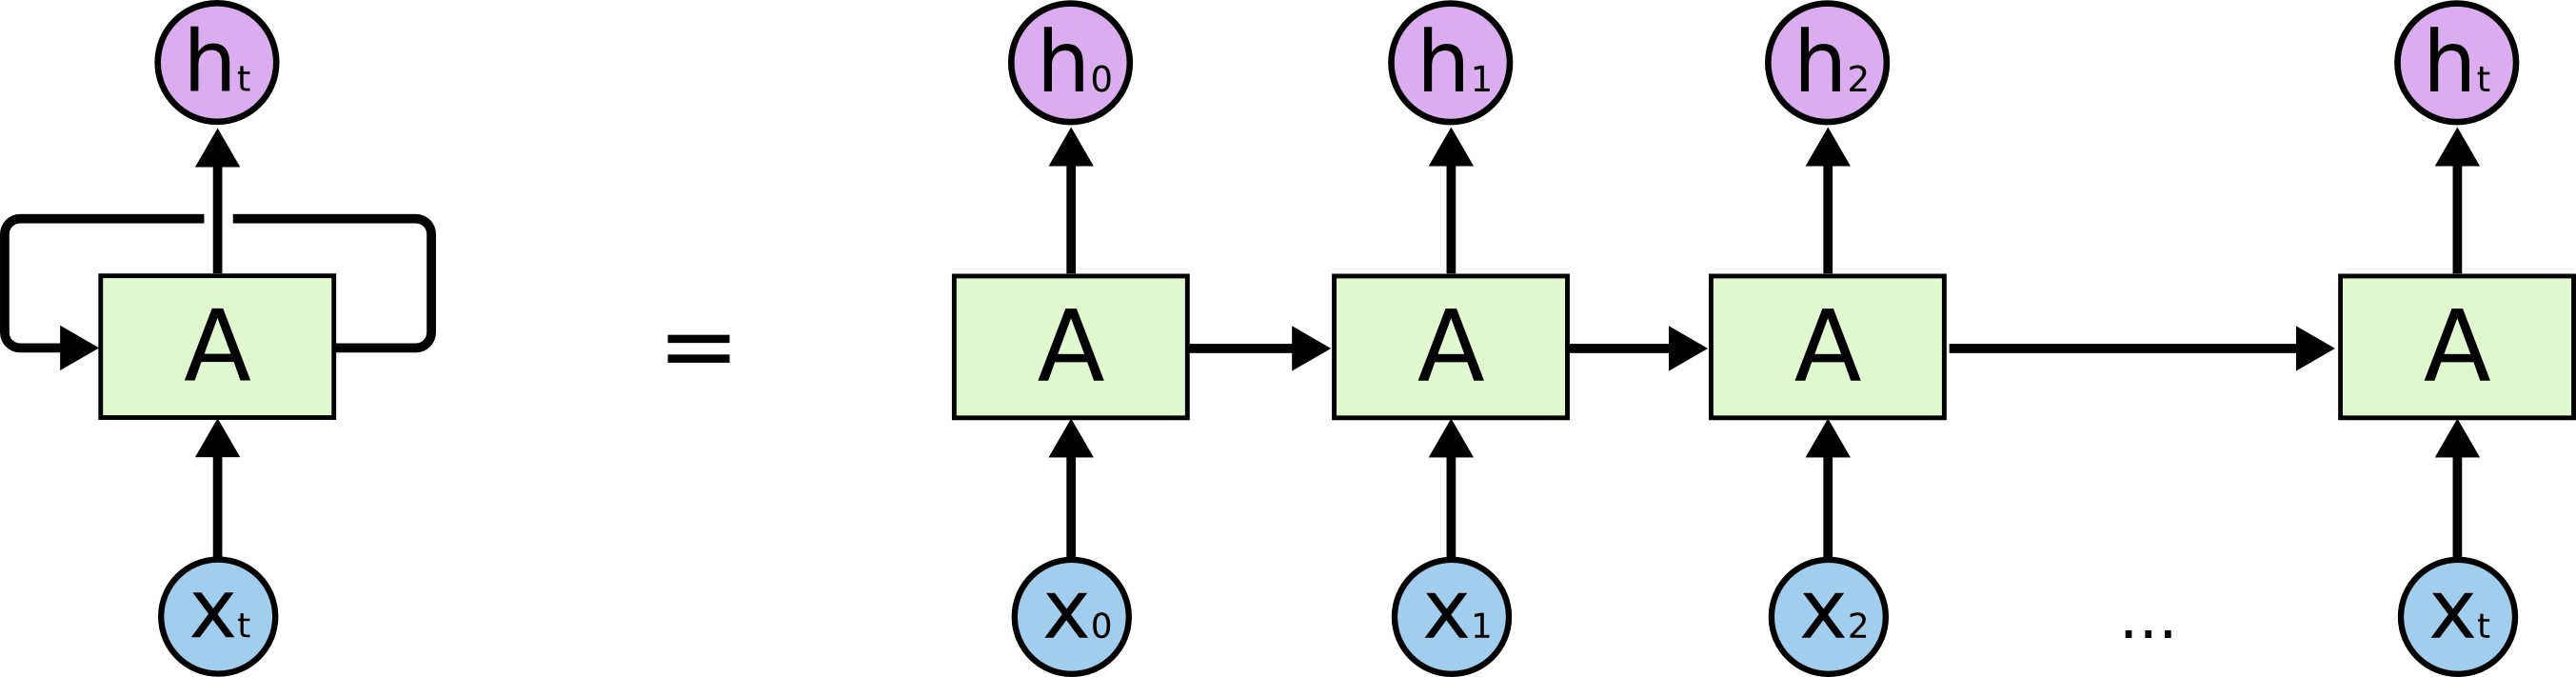
\includegraphics[width=0.8\textwidth, keepaspectratio]{RNN-unrolled}
    \caption{Схема рекуррентного слоя, где (слева)
    фрагмент нейронной сети $A$ принимает на вход некоторое значение $x_t$ 
    и возвращает некоторое значение $h_t$. Цикл позволяет информации 
    передаваться от одного шага сети к другому. Порой подобная 
    цикловая структура может сбить с толку, однак если его развернуть 
    (справа), то оказывается, что это очень похоже на классическую нейронную 
    сеть. О RNN можно думать как о множестве копий одной и той же сети, 
    каждая из которых передает сообщение своему последователю \cite{colah2}.}
    \label{fig:RNN-unrolled}
\end{figure}

Подобная цикловая структура позволяет обрабатывать последовательности 
данных произвольных размеров (стоит упомянуть, что в RNN мы используем 
одни и те же значения параметров (весов и смещений) 
внутри одного рекурентного слоя. Подобное разделение параметров позволяет 
применять и обобщать модель на примеры различной формы 
(в данном случае длины). Если бы у нас были различные параметры для 
каждого временного индекса, мы не смогли бы ни обобщить
модель на длины последовательностей, не встречавшиеся на этапе обучения, ни 
распространить статистическую силу на последовательности разной длины и 
на разные моменты времени).

% \subsubsection{Прямой проход}

% Прямой проход в RNN происходит по тому же принципу, что и в 
% многослойном перцептроне с одним скрытым слоем, за исключение того, что 
% активации поступают в скрытый слой как от текущего внешнего входа, так и 
% от активаций скрытого слоя, полученных на предыдущем временном шаге. 
% Рассмотрим последовательность входных данных $\bm{x}$ длины $T$, подающуюся 
% на вход RNN c $I$ входными блоками, $H$ скрытыми блоками и $K$ выходными 
% блоками. Пусть $x_i^t$ - значение входа $i$ в момент времени $t$, а 
% $a_j^t$ и $b_j^t$ - входное значение блока $j$ в момент времени $t$ и 
% активация блока $j$ в момент времени $t$ соответственно. Тогда, для 
% скрытых блоков имеем
% \begin{equation*}
%     a_h^t = \sum_{i=1}^I w_{ih} x_i^t + \sum_{h'=1}^H w'_{h'h} b_{h'}^{t-1},
% \end{equation*}
% (смещения были опущены для простоты)

% Нелинейные, дифференцируемые функции активации затем применяются точно так же, как 
% и в MLP:
% \begin{equation*}
%     b_h^t = \theta_h (a_h^t),
% \end{equation*}
% где $\theta_h$ - функция активации блока $h$

% Полная последовательность скрытых активация может быть получена, если принять 
% $t=1$ и затем рекурсивно применять две вышеописанные формулы, увеличивая $t$ 
% на каждом шаге. Заметим, что данный подход требует выбора начальных значений 
% для $b_i^0$ в скрытых блоках, соответствующих состоянию сети до того как 
% она получила какую либо информацию из входных данных. Часто это значение 
% выбирают равным 0. Однако некоторые исследователи заметили, что можно улучшить 
% стабильность и эффективность RNN выбрав ненулевые значения.

% Входные значения выходных блоков в сети могут быть посчитаны в тот же момент, что 
% и скрытые активации \cite{graves}:
% \begin{equation*}
%     a_k^t = \sum_{h=1}^H w_{hk} b_h^t
% \end{equation*}

% \newpage

% Рассмотрим пример. Пусть задана двумерная последовательность 
% (например ежедневные значения температуры и влажности) и T=2, I=2, H=3, K=2, 
% тогда развернутую схему рекуррентной сети можно представить в виде:
% \begin{figure}[h!]
%     \centering
%     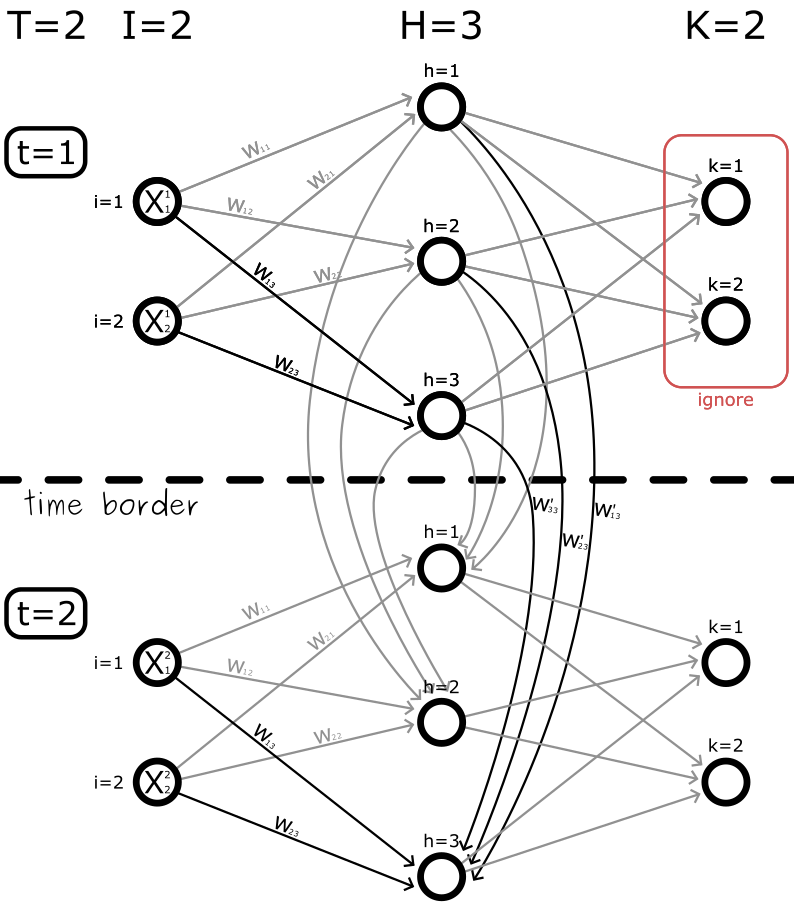
\includegraphics[width=0.8\textwidth, keepaspectratio]{RNN_unrolled_no_bg}
%     \caption{Пример RNN с выделенными весами для 
%     расчета одного рекуррентного блока. В случаях когда результаты 
%     выходных блоков в промежуточные моменты времени не требуются, их 
%     можно просто игнорировать, что и показано на рисунке.}
%     \label{fig:RNN_unrolled}
% \end{figure}

% Разумеется на практике чаще используют RNN, состояющие не из одного 
% рекуррентного слоя, а нескольких, чтобы получить, так называемые, 
% \textbf{глубокие рекуррентые нейронные сети (deep RNNs)}. Такой подход 
% позволяет нам, как и в случае многих слоев в FFNN и CNN, 
% обучить иерархические зависимости между признаками, что на практие 
% работает лучше однослойных сетей. 

% \subsubsection{Обратный проход}

% В силу своей природы, в RNN используется не классический метод обратного 
% распространения ошибки (backpropagation) 
% (см. главу {\color{red} todo}), а его модификация: 
% \textbf{метод обратного распространения ошибки во времени 
% (backpropagation through time (BPTT))} (разумеется существуют 
% и другие алгоритмы, например RTRL, но в данной работе мы сфокусируемся на 
% BPTT, тк он концепутально проще, популярнее и вычислительно эффективнее по времени 
% (но не по памяти)). Принцип работы у BPTT такой же, как и у 
% традиционного backprop. Единственное отличие заключается в том, что BPTT 
% суммирует ошибки в каждый момент времени, когда, сети прямого распространения, 
% в свою очердь, в этом не нуждаются, тк они не сохраняют значения параметров между 
% слоями.

\subsection{Вентильные RNN}

Одними из самых эффективных моделей последовательностей в практических 
приложениях считаются \textbf{рекуррентные нейронные сети с вратами 
(вентильные РНС (gated RNN))}. К ним относятся
\textbf{долгая краткосрочная память (long short-term memory - LSTM)} 
и сети, основанные на вентильных рекуррентных блоках. 

Полезно, чтобы сети умели как \textit{накапливать} информацию 
(например, свидетельства в пользу конкретного признака или категории) на 
протяжении долгого времени, так и \textit{забывать} ее после использования. 
Например, если последовательность состоит из подпоследовательностей 
и мы хотим, чтобы блок с утечкой накапливал свидетельства
внутри каждой подпоследовательности, то необходим механизм забывания старого
состояния - сброса его в нуль. И хорошо бы, чтобы нейронная сеть обучилась, 
когда это нужно делать, не обременяя нас принятием решения. 
Именно для этого и предназначены вентильные RNN.

\subsubsection{LSTM}

Важное преимущество RNN заключается в их возможности использовать 
контекст при сопоставлении входных и выходных последовательностей. 
К сожалению, для стандартных архитектур RNN диапазон допустимого контекста 
на практике весьма ограничен. Проблема заключается в том, что влияние 
заданной входной последовательности на скрытый слой, а следовательно и 
на выход сети либо затухает, либо экспоненциально взрывается по мере 
прохождения по рекуррентным связям сети. Эта проблема известна как проблема 
затухающего/взрывающегося градиента. Данная проблема особенно присуща 
рекуррентным нейронным сетям, т.к. напрямую зависит от размера рассматриваемой 
входной последовательности. Она исторически была одним из самых 
больших препятствий на пути к успеху рекуррентных нейронных сетей.

Можно было бы надеяться избежать этой проблемы, просто оставаясь в области пространства
параметров, где градиенты не затихают и не растут взрывообразно. К сожалению,
для хранения «воспоминаний» способом, устойчивым к малым возмущениям, RNN
должна войти в область пространства параметров, где градиенты исчезают.

\begin{figure}[h!]
    \centering
    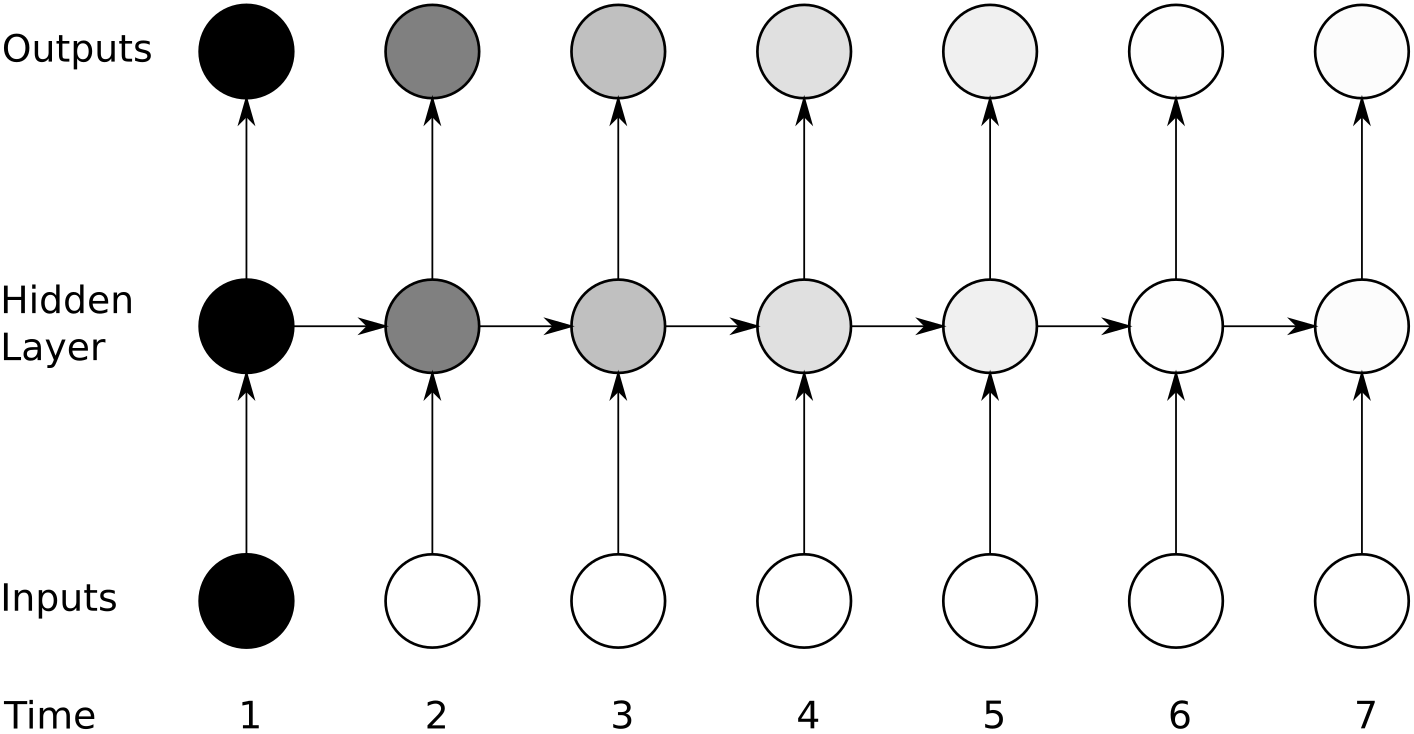
\includegraphics[width=0.8\textwidth, keepaspectratio]{RNN_vanishing_gradient}
    \caption{\textbf{Проблема затухающего градиента в RNN.} Затенение узлов в 
    развернутой сети указывает на их чувствительность ко входам в начальный момент 
    времени (чем темнее оттенок, тем выше чувствительность). Со временем 
    чувствительность снижается, т.к. новые входы затмевают активации 
    скрытого слоя и сеть «забывает» первоначальные значения \cite{graves}.}
    \label{fig:RNN_vanishing_gradient}
\end{figure}

С целью избежания именно этой проблемы был разработан особенный 
вид архитектуры рекуррентной нейронной сети, под названием 
\textbf{долгая краткосрочная память (Long Short Term Memory - LSTM)} (разработанная учеными 
Hochreiter \& Schmidhuber (1997) \cite{lstm}. Интересно, что именно Hochreiter 
изначально отрыл проблему затухающего градиента). Для большинства задач, требующих 
работы с последовательностями, LSTM работают гораздо лучше обычной версии. 
Почти что все захватывающие результаты в области рекуррентных нейронных 
сетей были достигнуты именно с их помощью. 

% LSTM

Все рекуррентные нейронные сети имеют вид, своего рода, цепочки 
повторяющихся модулей нейронной сети. В стандартных RNN, у этого 
повторяющегося модуля будет очень простая структура, 
например единственный слой с tanh.

\begin{figure}[h!]
    \centering
    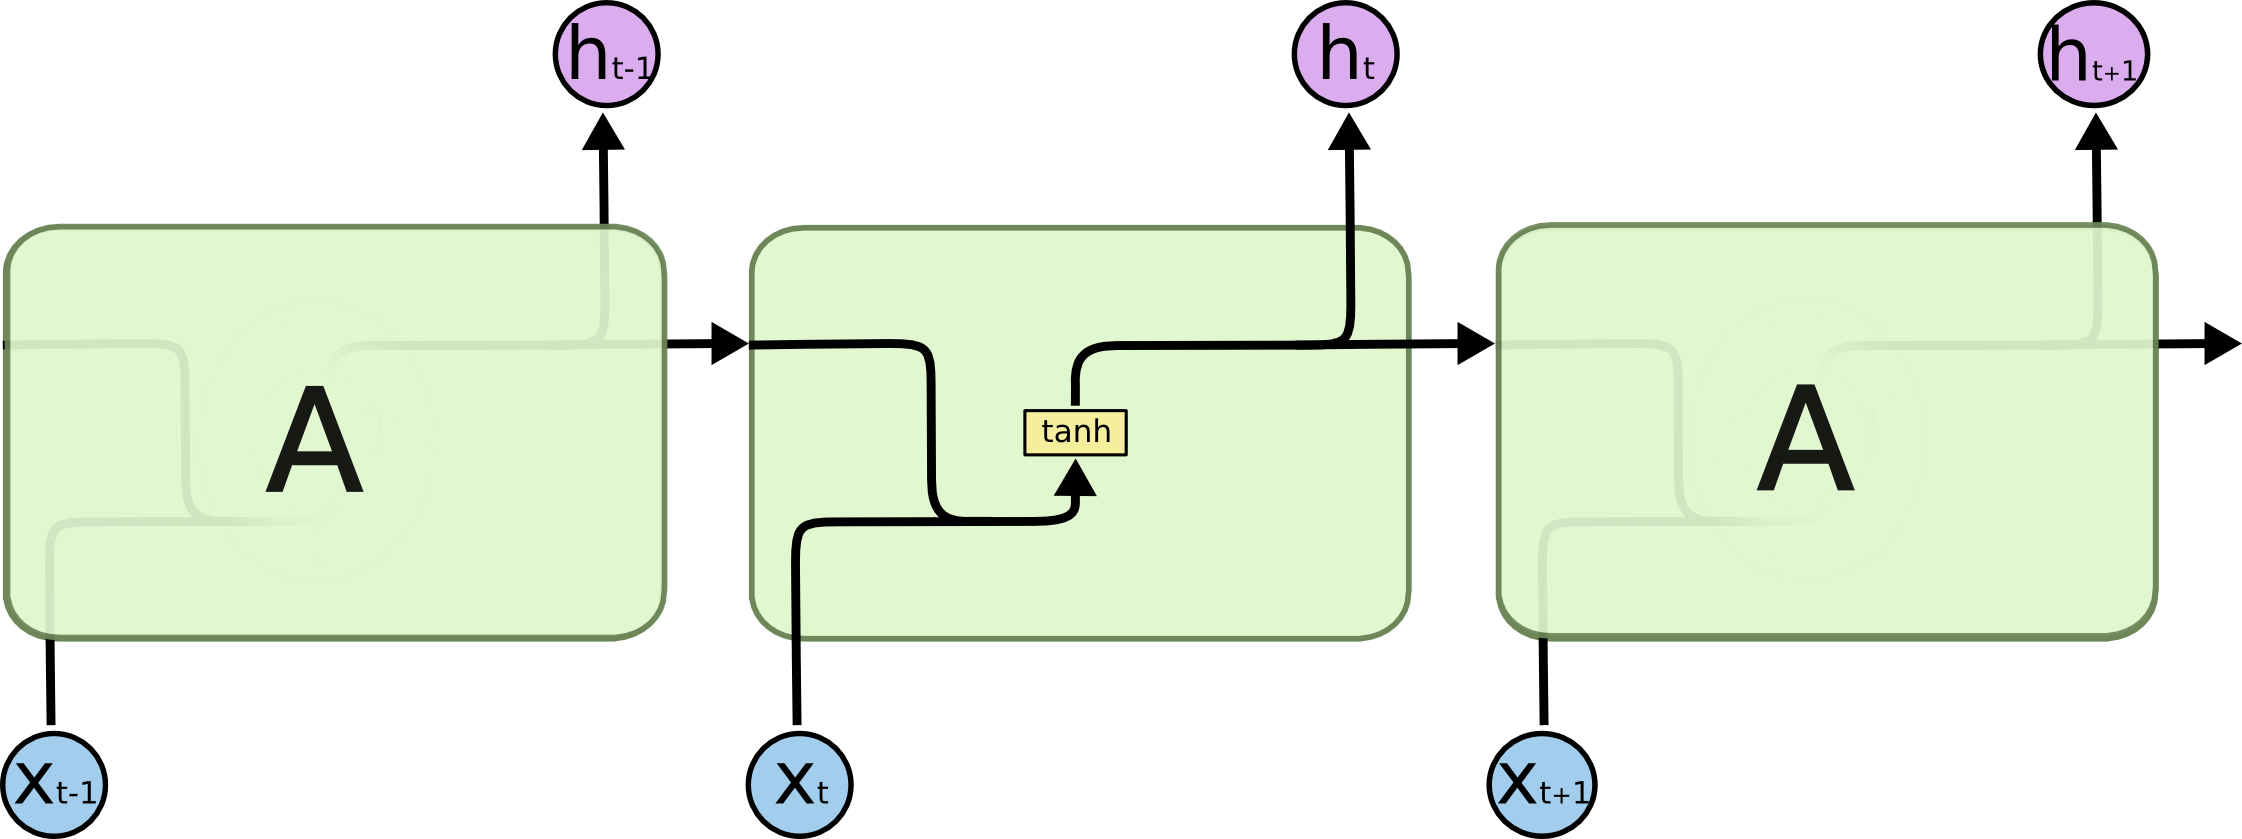
\includegraphics[width=0.8\textwidth, keepaspectratio]{RNN_tanh}
    \caption{Повторяющийся модуль в стандартной RNN, включающий 
    в себя единственный слой \cite{colah2}.}
    \label{fig:RNN_tanh}
\end{figure}

у LSTM, в свою очередь, тоже обладают подобной цепочкообразной структурой, 
но у повторяющегося модуля другая структура. Вместо единственного слоя 
нейронной сети, у него их четыре, все взаимодействующие друг с другом 
особенным образом. 

\begin{figure}[h!]
    \centering
    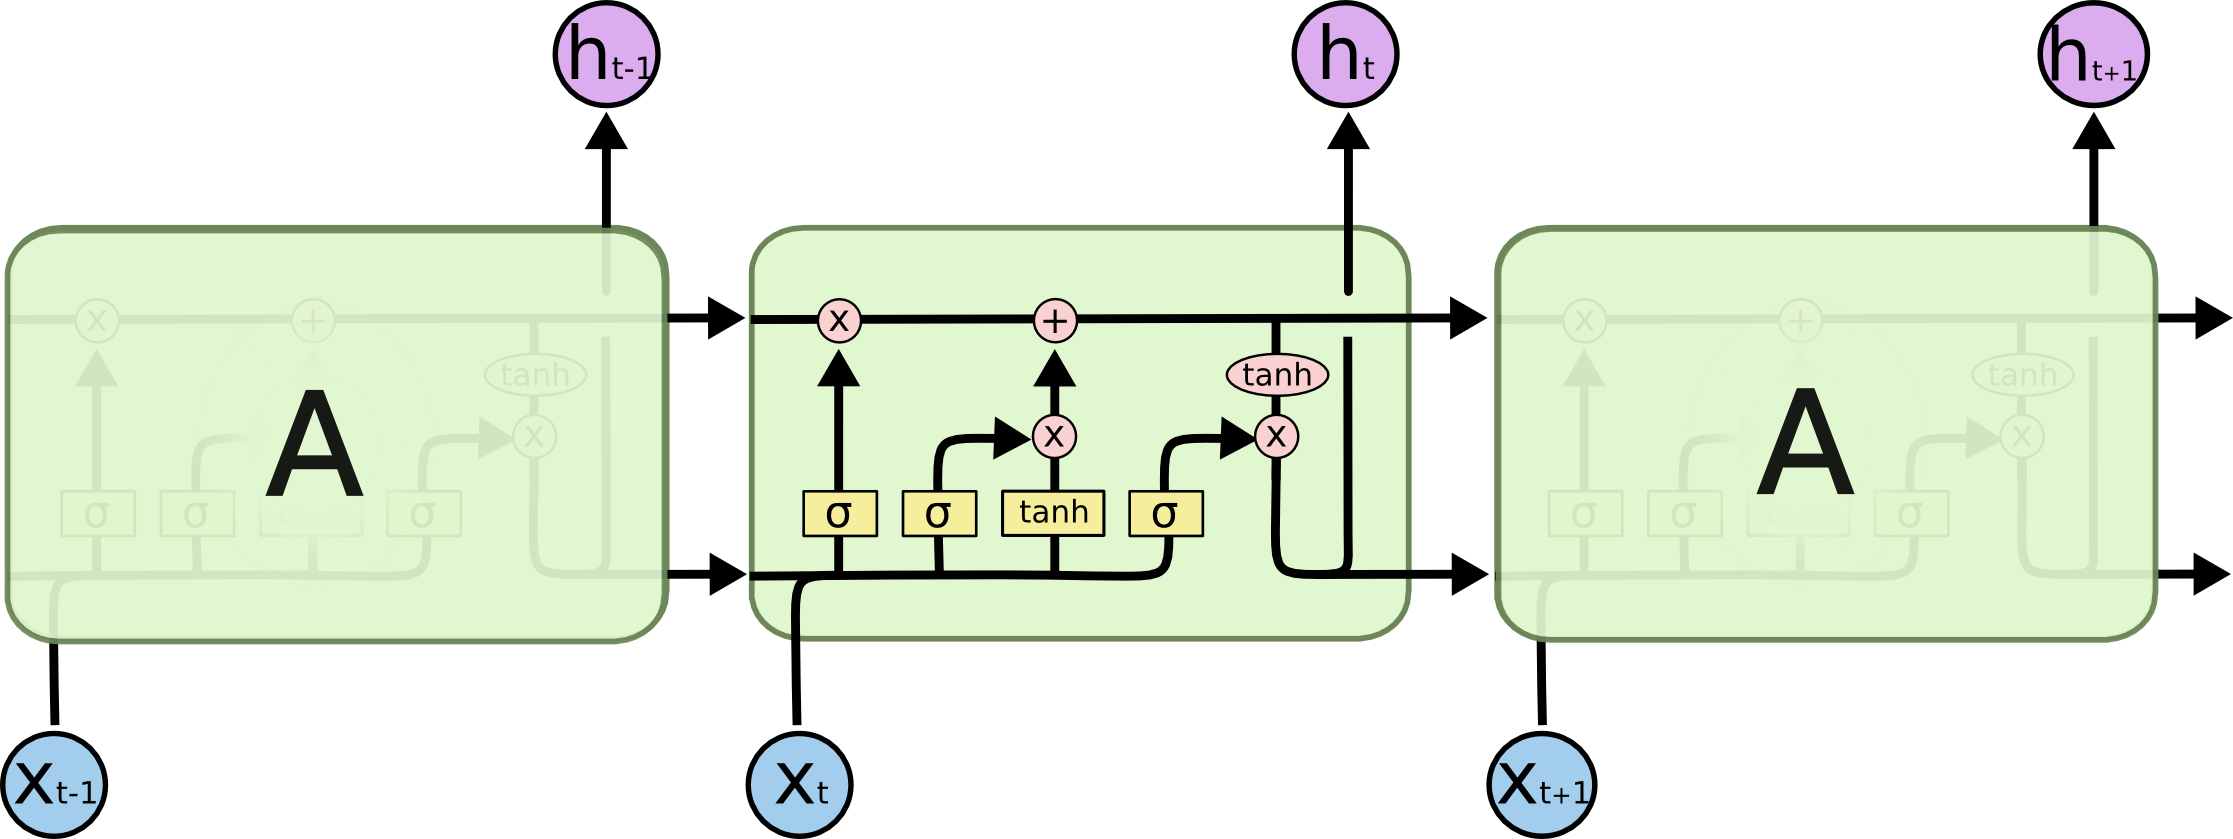
\includegraphics[width=0.8\textwidth, keepaspectratio]{RNN_LSTM}
    \caption{Повторяющийся модуль в LSTM, включающий 
    в себя четыре, взаимодействующих друг с другом слоя \cite{colah2}.}
    \label{fig:RNN_LSTM}
\end{figure}

Вместо блока, который просто применяет
поэлементную нелинейность к аффинному преобразованию входов и рекуррентным
блокам, в рекуррентных LSTM-сетях имеются «LSTM-ячейки», обладающие внут­ренней 
рекуррентностью (петлей) в дополнение к внешней рекуррентности RNN.
Об этих ячейках можно думать как о дифференцируемой версии чипов памяти в 
цифровом компьютере. Каждый блок содержит одну или более самосоединенных 
ячеек памяти и три мультипликативных блока - 
входные, выходные врата и врата забывания 
(the input, output and forget gates), которые предоставляют 
непрерывные аналоги операций записи, чтения и сброса для ячеек.

\begin{figure}[h!]
    \centering
    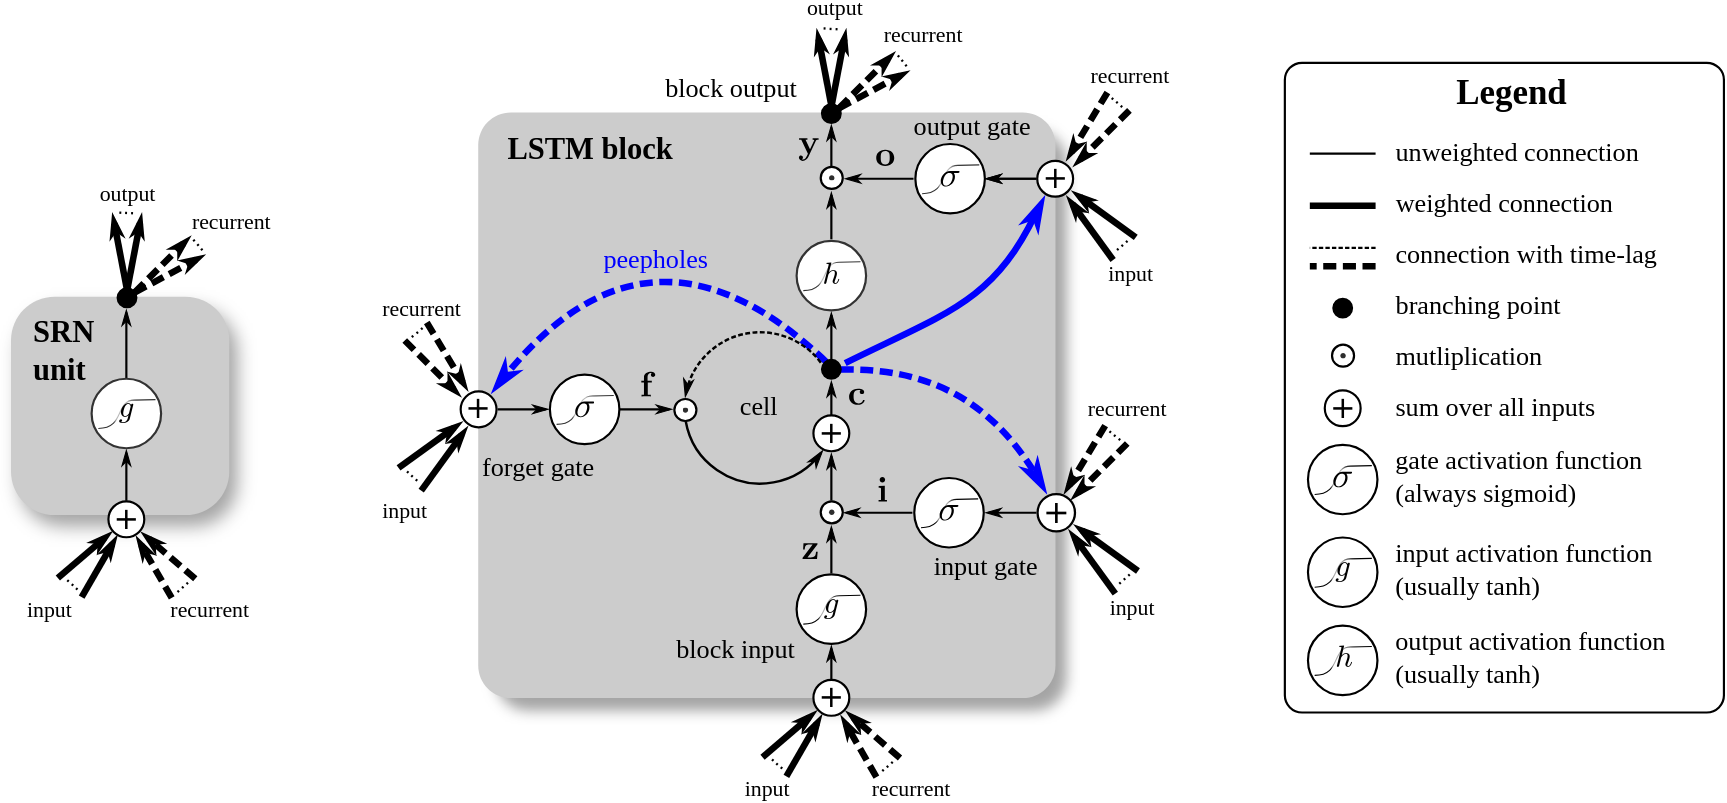
\includegraphics[width=1\textwidth, keepaspectratio]{LSTM_block}
    \caption{\textbf{Подробная схема блока простой рекуррентной нейронной сети 
    (Simple Recurrent Network - SRN) (слева) и блока LSTM (справа), 
    используемых в скрытых слоях рекуррентной нейронной сети \cite{greff2017lstm}.}
    Трое врат представляют из себя нелинейные суммирующие блоки, которые 
    собирают активации изнутри и снаружи основного блока и 
    управляют активацией ячейки через перемножения. Входные и выходные врата 
    умножают вход и выход ячейки, когда врата забывания, в свою очередь, 
    умножают предыдущее состояние ячейки. Внутри ячейки функция активации не 
    применяется. В качестве функции активации врат (gate activation function) 
    '$\sigma$' обычно используется логистическая сигмоида, чтобы 
    активации врат были между 0 (врата закрыты) и 1 (врата открыты). 
    В каечтсве функции активации входа и выхода ячейки (input activation function and 
    output activation function) ('$g$' и '$h$') обычно используется tanh 
    или логистическая сигмоида, хотя иногда '$h$' бывает и тождественным 
    преобразованием. Взвешенные «глазковые связи» (peepholes) от 
    ячеек к вратам изображены синим цветом. Единственные выходы из основного 
    блока в остальную часть сети проходят через перемножение выходных врат. 
    (Отметим, что данная схема несколько отличается от представленной 
    на рис. \ref{fig:RNN_LSTM} в силу, так называемых, «глазковых связей» 
    (peepholes), но мы не будем на них акцентировать внимание).}
    \label{fig:LSTM_block}
\end{figure}

Мультпликативные врата позволяют ячейкам памяти LSTM хранить и обращаться 
к информации через длительные временные промежутки, тем самым 
смягчая проблему затухающего градиента. Например, пока входные врата 
остаются закрытыми (т.е. их активация близка к 0), 
активация ячейки не будет перезаписана новыми входными данными, поступающими 
в сеть, и тем самым, может быть предоставлена сети гораздо позже в 
последовательности, путем открытия выходных врат. Сохранение информации о 
градиенте с течением времени в LSTM иллюстрировано на рис. \ref{fig:LSTM_vanishing_gradient}.

\begin{figure}[h!]
    \centering
    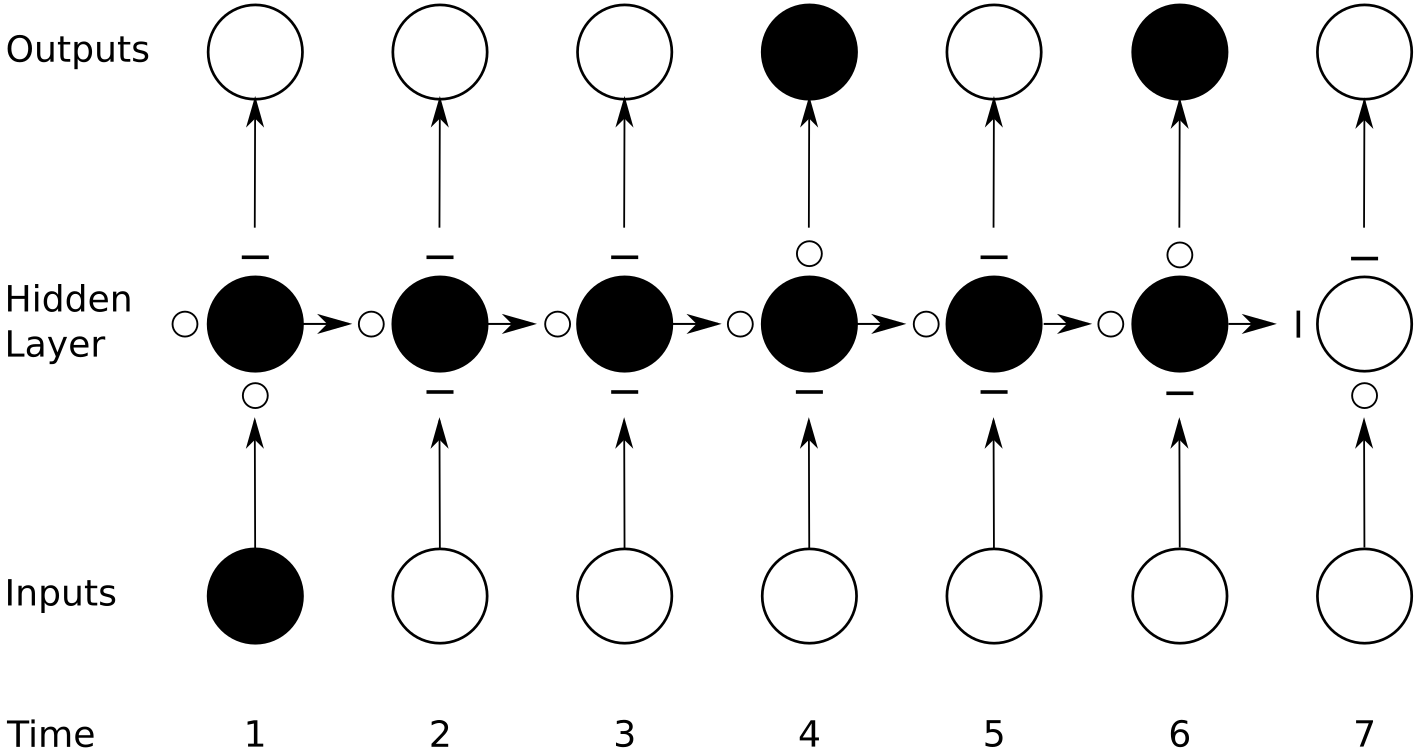
\includegraphics[width=0.8\textwidth, keepaspectratio]{LSTM_vanishing_gradient}
    \caption{\textbf{Сохранение информации о 
    градиенте с течением времени в LSTM.} Как и на рис. 
    \ref{fig:RNN_vanishing_gradient}, затенение узлов указывает на 
    их чувствительность ко входам в начальный момент времени; в 
    этом случае, черные узлы максимально чувствительны, а 
    белые узлы совершенно бесчувственны. Состояние 
    входных, выходных врат и врат забывания представлены 
    снизу, сверху и слева от скрытых слоев соответственно. Для 
    простоты, все врата либо полностью открыты ('O'), либо закрыты ('--'). 
    Ячейка памяти «помнит» первый вход до тех пор, пока врата забывания 
    открыты, а входные врата закрыты. Чувствительность выходного слоя 
    можно «включать» и «выключать» при помощи выходных врат без оказания 
    какого-либо влияния на ячейку \cite{graves}.}
    \label{fig:LSTM_vanishing_gradient}
\end{figure}

Формально, внутреннее состояние LSTM-ячейки $s_i^{(t)}$ обновляется по следующей 
формуле \cite{Goodfellow-et-al-2016}:
\begin{equation*}
    s_i^{(t)} = f_i^{(t)} s_i^{(t-1)} + g_i^{(t)} \sigma \left( 
        b_i + \sum_j U_{i,j} x_j^{(t)} + \sum_j W_{i,j} h_j^{(t-1)},
    \right)
\end{equation*}
где\vspace{-5pt}
\begin{gather*}
    f_i^{(t)} = \sigma \left( 
        b_i^f + \sum_j U_{i,j}^f x_j^{(t)} + \sum_j W_{i,j}^f h_j^{(t-1)}
    \right), \\[0.5em]
    g_i^{(t)} = \sigma \left( 
        b_i^g + \sum_j U_{i,j}^g x_j^{(t)} + \sum_j W_{i,j}^g h_j^{(t-1)}
    \right)
\end{gather*}
и
$s_i^{(t)}$ - блок состояния с линейной петлей, 
$f_i^{(t)}$ - врата забывания (для временного шага $t$ и ячейки $i$), 
которые управляет весом петли и присваивают ему значение от 0 до 1 с помощью 
сигмоиды,
$g_i^{(t)}$ - входные врата,
$\bm{x}^{(t)}$ - текущий входной вектор,
$\bm{h}^{(t)}$ - вектор текущего скрытого слоя, содержащий выходы всех LSTM-ячеек,
$\bm{b}^f, \bm{U}^f, \bm{W}^f$ - соответственно смещения, веса входов и рекуррентные веса для врат забывания,
$\bm{b}, \bm{U}, \bm{W}$ - соответственно смещения, веса входов и рекуррентные веса LSTM-ячейки. 

Выход $h_i^{(t)}$ LSTM-ячейки можно перекрыть с помощью выходных врат 
$q_i^{(t)}$, в которых также используется сигмоида:
\begin{align*}
    h_i^{(t)} &= \text{tanh}(s_i^{(t)})q_i^{(t)}, \\[0.5em]
    q_i^{(t)} &= \sigma \left( 
        b_i^o + \sigma_j U_{i,j}^o x_j^{(t)} + \sum_j W_{i,j}^o h_j^{(t-1)}
    \right),
\end{align*}
и $\bm{b}^o, \bm{U}^o, \bm{W}^o$ - смещения, веса входов и рекуррентные веса соответственно.

\subsubsection{GRU}

GRU представляет из себя упрощенную версию LSTM. \textbf{Входные} врата и врата 
\textbf{забывания} в них объединены в одни врата \textbf{обновления} (update gates), 
тем самым уменьшая количество параметров и делая модель менее вычислительно затратной.

Таким образом, GRU состоит из двух врат:
\begin{itemize}
    \item \textbf{Врата обновления (Update gate):} Отвечают за то, сколько информации из прошлого будет сохранено для будущих шагов. Они помогают GRU запоминать важные детали.
    \item \textbf{Врата сброса (Reset gate):} Отвечают за то сколько прошлой информации должно быть забыто. Если нам что то более не требуется, то эти врата помогают нам это забыть.
\end{itemize}

\begin{figure}[h!]
    \centering
    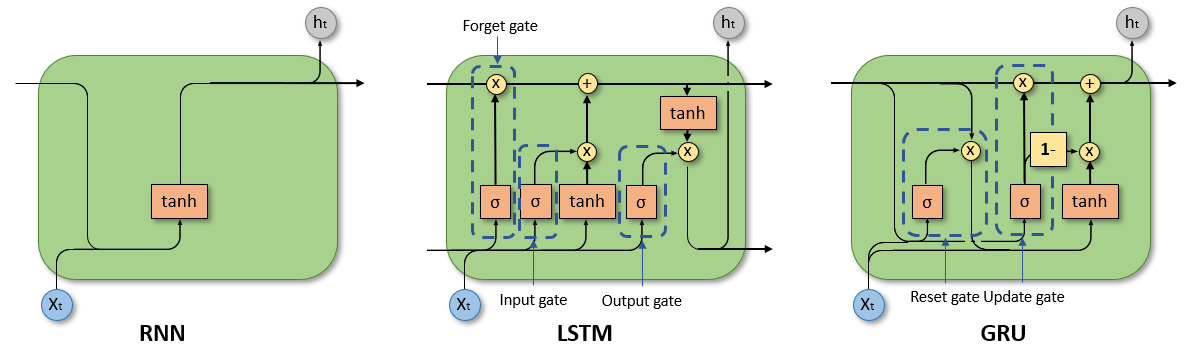
\includegraphics[width=1\textwidth, keepaspectratio]{GRU.png}
    \caption{Gated Recurrent Units (GRU).}
    \label{fig:GRU}
\end{figure}

Уравнения обновления имеют вид:
\begin{equation*}
    h_i^{(t)} = u_i^{(t-1)} h_i^{(t-1)} + (1-u_i^{(t-1)}) \sigma \left( 
        b_i + \sum_j U_{i,j} x_j^{(t-1)} + \sum_j W_{i,j} r_j^{t-1} h_j^{(t-1)}
    \right),
\end{equation*}
где $\bm{u}$ обозначает врата \textbf{обновления}, а $\bm{r}$ - врата \textbf{сброса}. 
Их значения определяются как обычно:
\begin{gather*}
    u_i^{(t)} = \sigma \left(
        b_i^u + \sum_j U_{i,j}^u x_j^{(t)} + \sum_j W_{i,j}^u h_j^{(t)}
    \right); \\[0.5em]
    r_i^{(t)} = \sigma \left(
        b_i^r + \sum_j U_{i,j}^r x_j^{(t)} + \sum_j W_{i,j}^r h_j^{(t)}
    \right).
\end{gather*}

Врата обновления и сброса могут «игнорировать» части вектора состояния. 
Врата обновления действуют как условные интеграторы с утечкой с линейной
функцией по любому измерению, т. е. могут либо скопировать вход (один конец 
сигмоиды), либо полностью проигнорировать его (противоположный конец), заменив
новым «целевым состоянием» (к которому интегратор с утечкой желает сойтись).
Врата сброса контролируют, какие части состояния использовать для вычисления 
следующего целевого состояния, и вносят дополнительный нелинейный эффект в 
соотношение между прошлым и будущим состояниями \cite{Goodfellow-et-al-2016}.

GRU предлагают хороший компромис между производительностью и эффективностью, 
порой превосходя LSTM в определенных задачах, будучи при этом быстрее и 
требуя меньше ресурсов. Они идеальны для ситуаций, где эффективность 
вычислений играют ключевую роль и не сильно жертвуют точностью.

\subsection{Модификации}

Ранее мы сказали (рис. \ref{fig:RNN-steps}), что изучение RNN и LSTM послужат нам 
переходными ступенями к пониманию трансформеров, и это правда, но на самом деле 
ступеней несколько больше. В настоящей главе мы рассмотрим две очень важные надстройки 
над RNN, которые оказали огромное влияние на изобретение трансформеров.

\begin{figure}[h!]
    \centering
    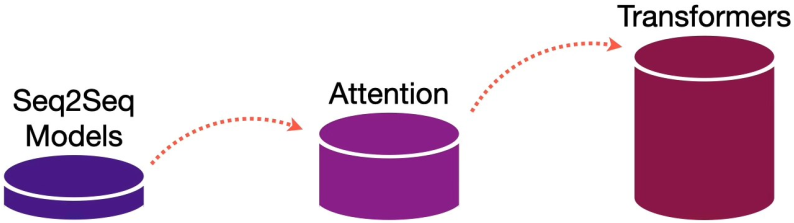
\includegraphics[width=0.8\textwidth, keepaspectratio]{RNN-steps2}
    \caption{\cite{statquest_ml_series}}
    \label{fig:RNN-steps2}
\end{figure}

% \subsubsection{\color{red}Bidirectional Long Short-Term Memory}

\subsubsection{Кодировщик-декодер}

В этом разделе мы рассмотрим, архитектуру RNN, способную отображать входную 
последовательность на выходную необязательно такой же длины. 
Такая задача возникает во многих
приложениях, например распознавании речи, машинном переводе и 
вопросно-ответных системах, где входные и выходные последовательности в 
обучающем наборе, вообще говоря, имеют разную длину 
(хотя их длины могут быть взаимосвязаны).

Вход такой RNN часто называют «контекстом». Мы хотим породить представление 
контекста $C$. Контекст $C$ может быть вектором или последовательностью векторов, 
агрегирующей входную последовательность $\bm{X} = (\bm{x}^{(1)}, ..., \bm{x}^{(n_x)})$.

Архитектура такого типа называется \textbf{кодировщик-декодер (encoder-decoder)} 
(рис. \ref{fig:encoder-decoder}) \cite{Goodfellow-et-al-2016}. 
Часто, особенно в задачах NLP, синонимично используется название 
последовательность в последовательность (sequence-to-sequence -- seq2seq), 
но строго говоря, понятие кодировщик-декодер более общее, тк 
допускает работу не только с последовательностями (например генерацию 
описания для изображения, т.е. изображение в последовательность). 

\begin{figure}[h!]
    \centering
    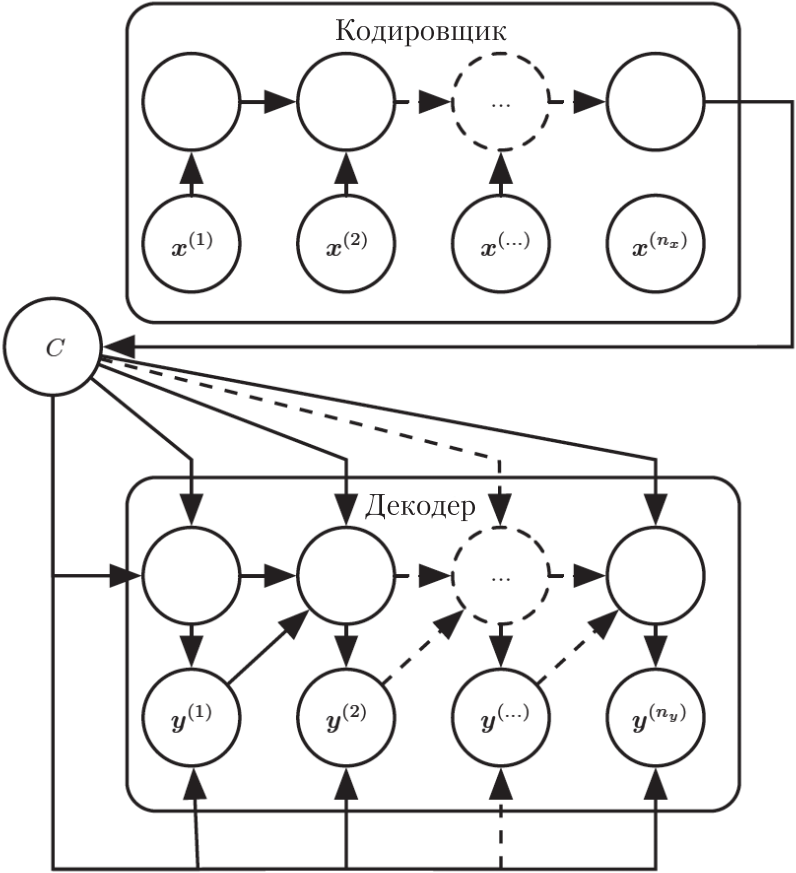
\includegraphics[width=0.5\textwidth, keepaspectratio]{encoder-decoder.png}
    \caption{Пример архитектуры RNN типа кодировщик-декодер, или
    последовательность в последовательность, которая обучается генерировать 
    выходную последовательность $\bm{y}^{(1)}, ..., \bm{y}^{(n_y)}$ по 
    входной последовательности $\bm{x}^{(1)}, \bm{x}^{(2)}, ..., \bm{x}^{(n_x)}$. 
    Сеть состоит из кодирующей RNN, которая читает
    входную последовательность, и декодирующей RNN, которая генерирует
    выходную последовательность (или вычисляет вероятность заданной выходной 
    последовательности). Конечное скрытое состояние кодирующей
    RNN используется для вычисления контекстной переменной $C$ фиксированного 
    размера, которая представляет собой семантическую сводку входной
    последовательности и подается на вход декодирующей RNN}
    \label{fig:encoder-decoder}
\end{figure}

\newpage

Модели, в которых имеются рекуррентные связи, идущие от выходов обратно в 
модель (что нередко практикуется при обучении моделей типа кодировщик-декодер), 
можно обучить методом \textbf{форсирования учителя (teacher forcing)}. Форсирование 
учителя - процедура, берущая начало в критерии максимального правдоподобия,
когда во время обучения модель получает истинную метку $y^{(t)}$ в качестве входа в 
момент $t + 1$ (после же обучения модель будет использовать свои собственные 
выходы в момент $t$ в качестве входов в момент $t + 1$).

Одной из работ, в которой изначально была предложена архитектура 
seq2seq считается статья \textbf{Sequence to Sequence Learning with Neural Networks} 
(Sutskever et al. (2014)) \cite{seq2seq} (мы говорим «одной из», тк независимо 
от данной работы, примерно в одно и тоже время были выпущены и другие, см. Cho et al. (2014), 
Bahdanau et al. (2014)). В данной работе на рассмотрение предлагается использование 
моделм LSTM, для построения архитектуры кодировщика-декодера 
(рис. \ref{fig:my-encoder-decoder}).

\begin{figure}[h!]
    \centering
    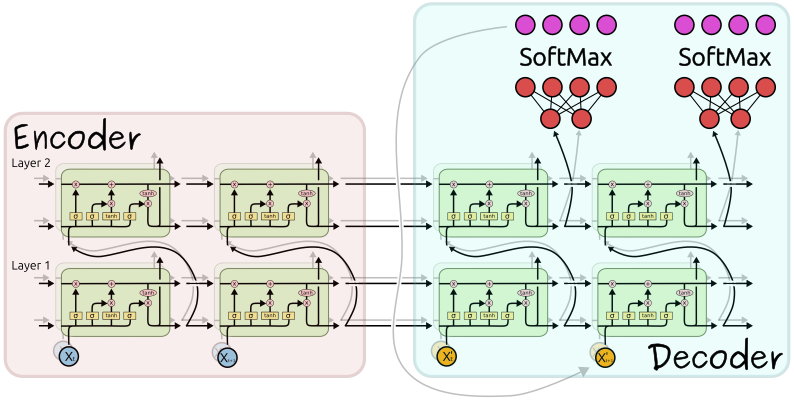
\includegraphics[width=1\textwidth, keepaspectratio]{my-encoder-decoder-no-bg.png}
    \caption{Пример упрощенной архитектуры seq2seq, предложенной в 
    \textbf{Sequence to Sequence Learning with Neural Networks} \cite{seq2seq} 
    (отметим, 
    что данная работа была нацелена на задачу машинного перевода, так 
    что строго говоря, на вход кодировщику и декодеру подаются, 
    так называемые, word embeddings, но мы не будем на этом акцентировать внимание). 
    Отметим также, что в оригинальной статье вместо нашего игрушечного входа в виде 
    последовательности из двух элементов используется словарь из 160000 токенов 
    для кодировщика и словарь из 80000 токенов для декодера. А вместо наших 
    2х слоев LSTM по 2 LSTM ячейки используются 4 слоя по 1000 LSTM ячеек в 
    каждом. Также у выходонго слоя не 2, а 1000 входов для каждой из 1000 LSTM 
    ячеек 4го слоя и 80000 выходов для соответствия выходного словаря.}
    \label{fig:my-encoder-decoder}
\end{figure}

\newpage

Очевидное ограничение этой архитектуры проявляется, когда размер контекста $C$,
порождаемого кодировщиком, слишком мал для формирования надлежащей сводки
длинной последовательности. Среди предложенных идей было введено понятие 
\textbf{механизма внимания}, 
который обучается ассоциировать элементы 
последовательности $C$ с элементами выходной последовательности.

\subsubsection{Механизм внимания}

Когда мы переводим предложение, то обычно обращаем особое внимание на текущее 
переводимое слово. Когда мы транскрибируем аудиозапись, то внимательно слушаем 
участок, который записываем. И если попросить человека описать комнату в которой он 
находится, то он пройдется глазами по предметам в комнате, 
по мере того как будет их описывать.

Нейронные сети могут добиться такого же поведения с помощью \textit{внимания}, 
фокусируясь на части подмножества информации, которая им предоставлена. 
Например, RNN может следить за выходом другой RNN. На каждом временном шаге 
она фокусируется на различных позициях в другой RNN (рис. \ref{fig:attention_mechs} (b)) 
\cite{olah2016attention}.

В своей работе \textbf{Neural Machine Translation By Jointly Learning To 
Align and Translate}, Bahdanau et al. (2015) предположили, 
что использование вектора фиксированной длины в моделе кодировщика-декодера 
является «бутылочным горшлышком» (bottleneck) при улучшении производительности 
и предложили расширирть ее, позволив модели автоматически осуществлять (soft-) 
поиск частей исходного предложения, которые имеют отношение к предсказанию целевого 
слова, без необходимости формировать эти части в виде жесткого сегмента в явном виде 
(что позже и получит название \textbf{механизма внимания (attention mechanism)})
\cite{attention_mech}.

Механзим внимания, использованный для фокусирования на отдельных частях выходного 
предложения на каждом временном шаге, иллюстрируется на рис. \ref{fig:attention_mechs} (a) 
\cite{Goodfellow-et-al-2016}.

\newpage

\begin{figure}[htbp]
    \centering
    \begin{minipage}{0.35\textwidth}
        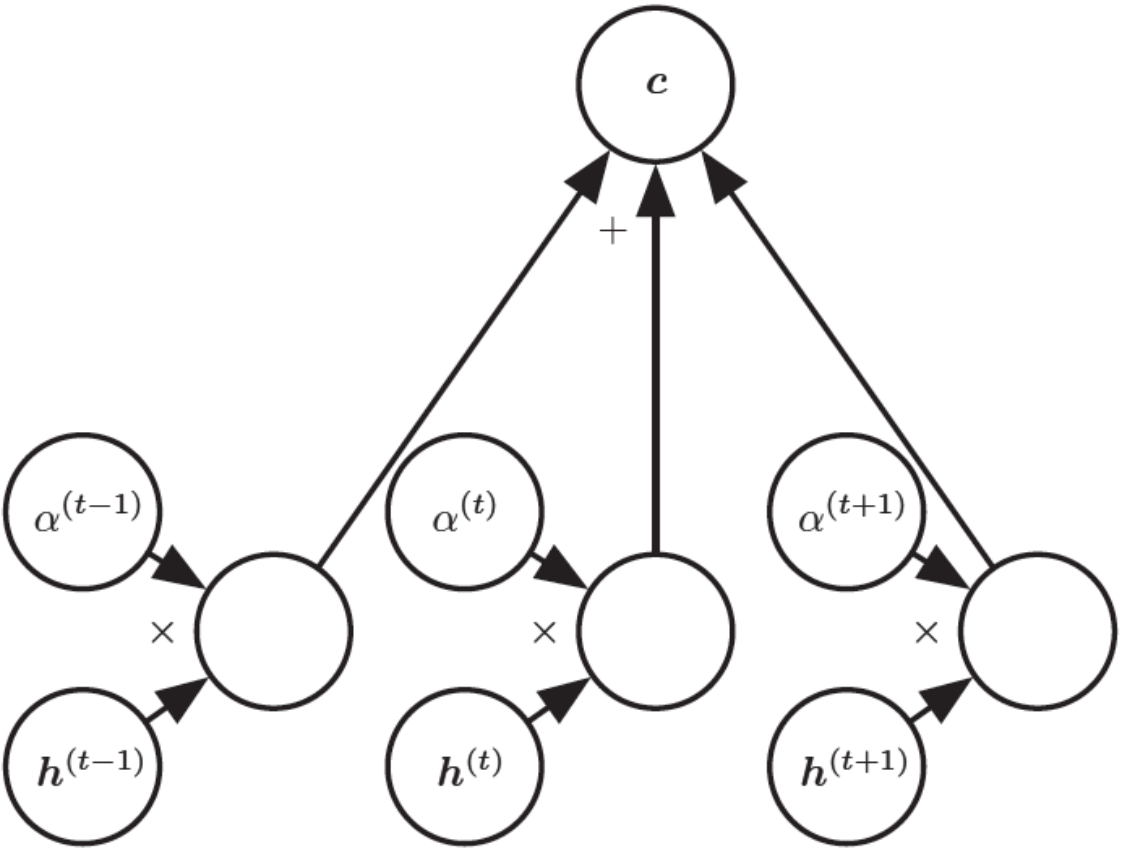
\includegraphics[width=\linewidth]{attention_mech1}
        \caption*{(a)}
        \label{fig:attention_mech1}
    \end{minipage}
    \hspace{30pt}
    \begin{minipage}{0.55\textwidth}
        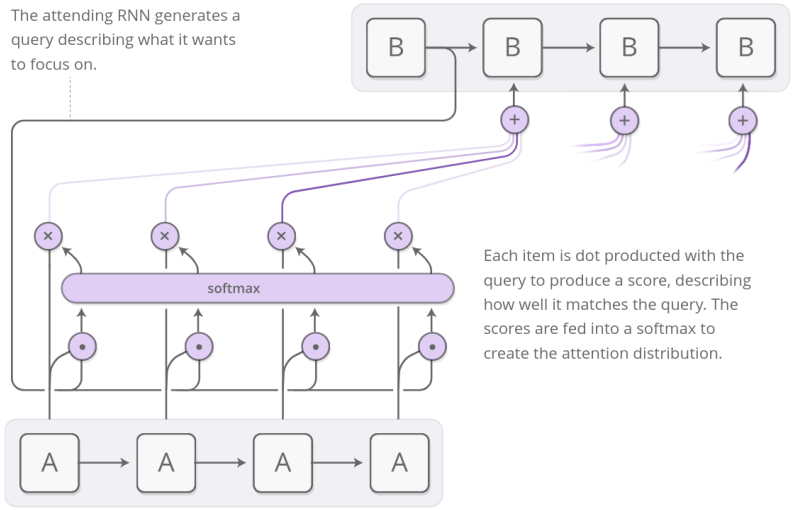
\includegraphics[width=\linewidth]{attention_mech2}
        \caption*{(b)}
        \label{fig:attention_mech2}
    \end{minipage}
    \caption{Современный механизм внимания, введенный в работе
    Bahdanau et al. (2015) \cite{attention_mech}, 
    по существу, представляет собой взвешенное
    среднее. Вектор контекста $\bm{c}$ образуется путем вычисления взвешенного
    среднего векторов признаков $\bm{h}^{(t)}$ с весами $\alpha^{(t)}$. 
    В некоторых приложениях
    векторы признаков $\bm{h}$ - скрытые блоки нейронной сети, но это могут быть
    и исходные данные модели. Веса $\alpha^{(t)}$ порождает сама модель. Обычно это
    значения из отрезка $[0, 1]$, которые концентрируются вокруг единственного
    значения $\bm{h}^{(t)}$, чтобы взвешенное среднее аппроксимировало чтение 
    именно на этом временном шаге. Как правило, веса $\alpha^{(t)}$ являются результатом
    применения функции softmax к оценкам релевантности, вычисленным другой 
    частью модели. Вычислительно механизм внимания дороже прямого
    индексирования желаемого $\bm{h}^{(t)}$, но прямому индексированию невозможно
    обучиться методом градиентного спуска. Механизм внимания, основанный
    на взвешенных средних, - гладкая дифференцируемая аппроксимация, допускающая 
    обучение существующими алгоритмами оптимизации \cite{Goodfellow-et-al-2016}.}
    \label{fig:attention_mechs}
\end{figure}

Отметим, что не смотря на различного рода соглашения, не существует единого правила 
того как именно интегрировать механизм внимания в архитектуру кодировщика-декодера. 
И в каждой работе это сделано по разному.

% TODO:
% Bidirectional Long Short-Term Memory
% Ensambles
